% Chapter Template

\chapter{Experiments and Evaluation}%
\label{chap:experiments_and_evaluation}

\section{Preparing Wordnets}%
\label{sec:preparing_wordnets}

In order to run our experiments we need two sets of dictionary definitions from two different languages.
Open Multilingual Wordnet~\cite{bond_linking_2013} project hosts 34 wordnets with permissive licenses on their website.\footnote{\url{http://compling.hss.ntu.edu.sg/omw}}
We have investigated the available wordnets and found out that six of them included definitions, also known as glosses.
Since we do not use any other information related to wordnets (like semantic relationships) only definitions were extracted into a plain text corpora.
This intermediate corpora includes WordNet 3.0 synsets identifiers and the corresponding definitions in the target language.
Natural Language Toolkit~\cite{bird_natural_2009} provides an API for reading and retrieving English Princeton WordNet.
Using the synsets identifiers, it is possible to retrieve the exact synset which comes attached with an unique definition.
Finally, we have 6 aligned corpora for 6 wordnets we will run the experiments on.
Alignment here refers to definitions that represent same synset across languages appearing on the same index or on the same line in their respective files.
Throughout the chapter, we will base our evaluations on these alignments.
The statistics and the 2 letter language codes that we will commonly use to denote the wordnets for the chapter is presented in Table~\ref{tab:wordnet_stats}.

\begin{table}[hbtp]
    \centering
    \settowidth\tymin{\textbf{Language}}
    \setlength\extrarowheight{2pt}
    \begin{tabulary}{1.0\linewidth}{L L R R R R}
        \toprule
        \textbf{Language Code} & \textbf{Language Name} & \textbf{Number of Definitions} & \textbf{Number of words} & \textbf{Average Words per Definition} & \textbf{Longest Definition} \\ \midrule
        sq & Albanian & 4681 & 54980 & 11.75 & 101 \\
        bg & Bulgarian & 4959 & 63014 & 12.71 & 53 \\
        el & Greek & 18136 & 203924 & 11.24 & 89 \\
        it & Italian & 12688 & 93005 & 7.33 & 35 \\
        ro & Romanian & 58754 & 586304 & 9.98 & 105 \\
        sl & Slovene & 3144 & 39865 & 12.68 & 68 \\
        \bottomrule
    \end{tabulary}%
    \caption{Language codes and statistics for the target wordnets used in the thesis.}%
    \label{tab:wordnet_stats}
\end{table}

\section{Preparing Word Embeddings}%
\label{sec:preparing_word_embeddings}

In Chapter~\ref{chap:background_n_related}, we have mentioned the recent popularization of pre-trained word embeddings.
Initiated by word2vec\footnote{\url{https://code.google.com/archive/p/word2vec}}, other sources for word embeddings are GloVe\footnote{\url{https://nlp.stanford.edu/projects/glove}}, fastText\footnote{\url{https://fasttext.cc}} and numberbatch\footnote{\url{https://github.com/commonsense/conceptnet-numberbatch}}.
Yet, word embeddings for languages other than English are scarce.
fastText hosts word embeddings for 157 languages so we used them as our primary source~\cite{grave_learning_2018}.
Numberbatch is another approach for word embeddings and \textcite{speer_conceptnet_2017} host word embeddings for 78 different languages.
Their embeddings are built on GloVe and word2vec and their model was explained in detail in Subsection~\ref{sub:conceptnet_numberbatch}.
However, 10 of the available languages are presented as core languages with excellent support and 68 of them are provided as common languages which are only available with adequate support.
Referring to Table~\ref{tab:wordnet_stats}, Italian is among the core languages and the rest are in the common languages group.
We provide their models as additional comparison.

These embeddings are trained using Common Crawl and Wikipedia data, on billions of tokens.
The lack of other embeddings models like GloVe in our study stems from the fact that downloading those huge corpora and training multilingual embeddings is a slow and expensive process.

The fastText embeddings include 2 million tokens out of the box.
In order to increase the efficiency of the experiments, we have cut down the size of the embeddings into 1 million and 500 thousand while learning bilingual word embeddings.
The vectors are sorted according to their corpus frequency so the uppermost lines where the most frequent tokens of the language reside are used.
For the rest of the chapter, while presenting the evaluation results, the distinction between fastText vectors with 1 million tokens and 500 thousand tokens will be shown as \emph{fastText 1M} and \emph{fastText 500k} respectively.

Numberbatch embeddings are distributed in one large file and vectors are not in a set size across languages.
Hence after parsing the file and extracting the embeddings into individual files, the number of word vectors we are left with are presented in Table~\ref{tab:numberbatch_stats}.

\begin{table}[hbtp]
    \centering
    \begin{tabulary}{1.0\linewidth}{L R}
        \toprule
        \textbf{Language Code} & \textbf{Number of Tokens} \\
        \midrule
        bg & 20871 \\
        el & 16926 \\
        en & 417195 \\
        it & 91829 \\
        ro & 10874 \\
        sl & 11458 \\
        sq & 5512 \\
        \bottomrule
    \end{tabulary}
    \caption{The number of word embeddings available in numberbatch}%
    \label{tab:numberbatch_stats}
\end{table}

These embeddings are monolingual, so they are on separate arbitrary latent spaces.
In order to represent them on the same latent space, we used VecMap~\cite{artetxe_robust_2018,artetxe_generalizing_2018,artetxe_learning_2017,artetxe_learning_2016}.\footnote{\url{https://github.com/artetxem/vecmap}}
According to \textcite{ruder_survey_2017}, bilingual or cross lingual embedding models optimize similar objectives and differences in performance is due to the data they are trained on.
\textcite{glavas_how_2019} supports this suggestion and has empirically proven that common evaluation metrics like bilingual dictionary induction is not representative for the bilingual embedding's performance on downstream tasks.
Hence our preference of VecMap is highly influenced by it's availability as an open source framework and it's ease of training.

Best performing VecMap model for learning bilingual embeddings that is available in the framework is \emph{supervised alignment}.
It requires a bilingual dictionary, otherwise known as aligned word pairs for two languages.
We sourced our bilingual dictionary from Open Subtitles 2018\footnote{\url{http://www.opensubtitles.org}} data as hosted by OPUS.\footnote{\url{http://opus.nlpl.eu}}
The dictionary can be sorted by the confidence score of the translation pair, which we did so that pairs with high confidence scores swam to the top.
Topmost 25000 translation pairs were shuffled and split into training and testing examples for 6 languages.
After supervised mapping of target language word embedding and English word embedding, we have 6 pairs of vectors that share the same latent space per pair, trained on 12500 word alignments.

\begin{table}[htbp]
    \centering
    \begin{tabulary}{1.0\linewidth}{L R R R}
        \toprule
        \textbf{Language Code} & \textbf{fastText 1M} & \textbf{fastText 500k} & \textbf{numberbatch} \\
        \midrule
        bg & 33.61 & 35.17 & 51.97 \\
        el & 37.37 & 39.58 & 30.35 \\
        it & 58.20 & 59.28 & 50.37 \\
        ro & 37.33 & 38.71 & 64.17 \\
        sl & 21.42 & 22.91 & 74.74 \\
        sq & 24.46 & 25.36 & 58.63 \\
        \bottomrule
    \end{tabulary}
    \caption{Accuracy scores (in percentage) of the word embeddings aligned using VecMap}%
    \label{tab:accuracy_results}
\end{table}

\begin{table}[htbp]
    \centering
    \begin{tabulary}{1.0\linewidth}{L R R R}
        \toprule
        \textbf{Language Code} & \textbf{fastText 1M} & \textbf{fastText 500k} & \textbf{numberbatch} \\
        \midrule
        bg & 96.43 & 93.36 & 17.53 \\
        el & 94.44 & 90.28 & 12.15 \\
        it & 97.93 & 95.97 & 41.08 \\
        ro & 97.06 & 94.91 & 16.4 \\
        sl & 94.67 & 90.73 & 9.23 \\
        sq & 83.59 & 80.92 & 9.51 \\
        \bottomrule
    \end{tabulary}
    \caption{Coverage scores (in percentage) of the word embeddings aligned using VecMap}%
    \label{tab:coverage_results}
\end{table}

Even though bilingual dictionary induction is not representative of a bilingual word embedding pair's performance on downstream tasks~\cite{ruder_survey_2017,glavas_how_2019}, we include the evaluation results obtained from VecMap framework as a quick identifier for their performance on Table~\ref{tab:accuracy_results} for accuracy and Table~\ref{tab:coverage_results} for coverage.
Accuracy is the measure for correctly identifying the translation of a word given the test dictionary and coverage is the percentage of translation pairs that could be inducted.
From the results, it is apparent that fastText embeddings have much better coverage due to vast data they were trained on.
Yet, numberbatch exhibits better accuracy scores which might be a trade-off of their low coverage.
Also note that Italian, which is the sole language in our experiment set which numberbatch claims to have full support for has significantly higher coverage score compared to rest of the languages.
Nevertheless, bilingual dictionary induction results are not indicative of word embedding's performance on real life tasks.

\section{Experiment Results}%
\label{sec:results}

In this section, we will present the results of our experiments in the order they appeared in the main text of our study.
Then, we will compare the approaches by presenting their results when ran on equivalent data.

\subsection{Matching Results}%
\label{sub:matching_results}

To begin with, we evaluated linear assignment or matching approach using sentence embeddings and cosine similarity as the similarity measure between definitions.
Using the graph analogy, nodes of the disjoints sets are dictionary definitions of two languages and edge weights between the nodes are the cosine similarity between the definitions across languages.
Linear assignment algorithm proposed by \textcite{jonker_shortest_1987} optimizes the overall cost of the bijection.
This approach is presented in detail at Section~\ref{sec:linear_assignment_using_sentence_embeddings}.
Since linear assignment is a one-to-one operation, we report precision at one or the percentage of definitions that are matched correctly.

The terms that do not have word embeddings available in the models are dropped from the definitions.
If a definition falls shorter than 3 words after this operation, it is dropped from the experiment set completely.
As a result, we report \emph{cardinality}, the number of definitions available on two languages.
Linear assignment using sentence embeddings using all of the available dictionary definitions per language is presented at Table~\ref{tab:lapjv_sentence_emb}.

\begin{table}[htbp]
    \centering
    \begin{tabulary}{1.0\linewidth}{L L R R}
        \toprule
        \textbf{Language Code} & \textbf{Vector} & \textbf{Cardinality} & \textbf{Precision at one \%} \\ \midrule
        \multirow{3}{*}{bg} & fastText 1M & 4958 & 27.93 \\
                            & fastText 500k & 4958 & 28.52 \\
                            & numberbatch & 4896 & 12.99 \\
        \multirow{3}{*}{el} & fastText 1M & 18117 & 31.15 \\
                            & fastText 500k & 18105 & 31.06 \\
                            & numberbatch & 17595 & 7.97 \\
        \multirow{3}{*}{it} & fastText 1M & 12590 & 15.50 \\
                            & fastText 500k & 12585 & 15.73 \\
                            & numberbatch & 12563 & 20.63 \\
        \multirow{3}{*}{sl} & fastText 1M & 3143 & 10.44 \\
                            & fastText 500k & 3143 & 11.42 \\
                            & numberbatch & 2955 & 4.70 \\
        \multirow{3}{*}{sq} & fastText 1M & 4680 & 44.96 \\
                            & fastText 500k & 4680 & 44.81 \\
                            & numberbatch & 4639 & 16.06 \\
                            \bottomrule
    \end{tabulary}
    \caption{Evaluation results for linear assignment using sentence embeddings}%
    \label{tab:lapjv_sentence_emb}
\end{table}

Romanian wordnet definitions did not fit into the memory of the machine we tested on so we could not present the full definition matching results for Romanian wordnet.
In order to show a complete picture, the experiments are done on 3000 definition pairs per language which are presented in Table~\ref{tab:lapjv_3000}.

\begin{table}[htbp]
    \centering
    \begin{tabular}{lrrr}
        \toprule
& \multicolumn{3}{c}{Percentage of Correctly Matched Definitions} \\
\cmidrule(lr){2-4}
        \textbf{Language Code} & \textbf{fastText 1M} & \textbf{fastText 500k} & \textbf{Numberbatch} \\
        \midrule
        bg & 35.27 & \textbf{36.00} & 18.10 \\
        el & \textbf{36.13} & 36.07 & 11.70 \\
        it & 24.67 & 24.90 & \textbf{32.07} \\
        ro & 36.43 & \textbf{36.87} & 18.73 \\
        sl & 11.27 & \textbf{11.40} & 4.63 \\
        sq & 39.43 & \textbf{39.67} & 19.03 \\
        \bottomrule
    \end{tabular}
    \caption{Definition matching evaluated on 3000 definition pairs}%
    \label{tab:lapjv_3000}
\end{table}

From Table~\ref{tab:lapjv_3000}, we can infer that fastText vectors truncated to 500 thousand tokens perform better overall while numberbatch is highly successful comparatively on the language it advertises full support for.

% \begin{table}[htbp]
%     \centering
%     \begin{tabular}{@{}lrrr@{}}
%         \toprule
%  & \multicolumn{3}{l}{Percentage of Correctly Matched Definitions} \\ \cmidrule(l){2-4}
%  & \textbf{fastText 1M} & \textbf{fastText 500k} & \textbf{Numberbatch} \\ \midrule
%         \textbf{Best} & 54.85 & 54.15 & 36.30 \\
%         \textbf{Worst} & 11.27 & 11.40 & 4.63 \\
%         \textbf{Average} & 32.93 & 33.35 & 18.92 \\
%         \bottomrule
%     \end{tabular}
%     \caption{The summary of matching dictionary definitions}%
%     \label{tab:lapjv_summary}
% \end{table}

% \begin{table}[htbp]
%     \centering
%     \begin{tabulary}{0.8\linewidth}{L r R}
%         \toprule
%         \textbf{Language Code} & \textbf{Definitions} & \textbf{Percentage of Definitions Matched Correctly} \\ \midrule
%         bg & 4958 & 28.52 \\
%         el & 18105 & 31.06 \\
%         it & 12585 & 15.65 \\
%         sl & 3143 & 11.42 \\
%         sq & 4680 & 44.81 \\
%         \bottomrule
%     \end{tabulary}
%     \caption{Definition matching using all the available definition in the corpora}%
%     \label{tab:lapjv_full}
% \end{table}

\subsection{Google Translate Baseline}%
\label{sub:chap4_results}

We have presented our method of translating the target wordnet definitions into English using Google Translate and running monolingual document retrieval on the corpora in Section~\ref{sec:monolingual_retrieval}.
As mentioned before, we used the original English definitions extracted from English Princeton WordNet as the document collection to retrieve from and used the translated target wordnet definitions as queries to retrieve with.
The experiments are done on 2000 definitions pairs for both languages.

The results are presented in Table~\ref{tab:google_translate_baseline}.
\tfidf{} weighted term document matrices and cosine similarity between definitions provide adequate results considering the simplicity of the approach.
However, we should consider mean reciprocal rank.
MRR penalizes the query according to the rank of the correct result, as the correct definition is retrieved on a lower rank, the MRR diminishes.
The divide between the MRR score and the precision at one score indicates that machine translation introduces noise that keeps the correct definition from appearing among the top results heavily for the majority of the cases.
We can draw attention to this fact by referring to Table~\ref{tab:google_translate_lol}.
In the said table, we have shown examples of erronous sentence structures and usage of words that are semantically similar to their translation sources but does not make sense from a native speaker's standpoint.
Such errors stem from machine translations and since Google Translate is a proprietary software, we cannot draw conclusions from the inner workings of it, but only point at the results available to us.

\begin{table}[htbp]
    \centering
    \begin{tabulary}{1.0\linewidth}{L R R R}
        \toprule
        \textbf{Language} & \textbf{MRR \%} & \textbf{Top 10 \%} & \textbf{Top 1 \%} \\ \midrule
        bg & 8.73 & 33.70 & 20.15 \\
        el & 12.22 & 50.30 & 35.45 \\
        it & 1.60 & 23.80 & 12.50 \\
        ro & 5.07 & 49.40 & 36.40 \\
        sl & 7.30 & 29.20 & 15.85 \\
        sq & 5.56 & 48.95 & 38.35 \\ \bottomrule
    \end{tabulary}
    \caption{Evaluation results of Google Translate baseline}%
    \label{tab:google_translate_baseline}
\end{table}

\subsection{Cross Lingual Document Retrieval Results}%
\label{sub:cross_lingual_retrieval_results}

We present the results of the two methods we have explained in detail at Section~\ref{sec:cross_lingual_document_retrival}.
Similar to how we built sentence embeddings, out of vocabulary words are handled simply by omitting them from the experiment data.
Any individual definition that does not have at least 3 tokens are removed from the experiment set alongside its equivalent on the other language.
We have chosen to remove 3 tokens arbitrarily, in order to remove potentially unrepresentative definitions as well as in order to keep the problem on the short document retrieval domain.

Cross lingual document retrieval is expensive in terms of memory requirements; in the study where the approach is proposed~\cite{balikas_cross-lingual_2018} as well as the open source implementation by the original author\footnote{\url{https://github.com/balikasg/WassersteinRetrieval}} which we modified for our study, the experiment set was kept at 500 documents on each language.
So, after removing the definitions according to the guidelines above, 2000 definitions on both languages are chosen randomly as the experiment data.

We present mean reciprocal scores in Table~\ref{tab:cldr_mrr} and precision at one scores in Table~\ref{tab:cldr_pao}.

\begin{table}[htbp]
    \centering
    \begin{tabulary}{1.0\linewidth}{L l R R R R}
        \toprule
        Language Code & \textbf{Vector} & \textbf{WMD tfidf} & \textbf{Sinkhorn tfidf} & \textbf{WMD tf} & \textbf{Sinkhorn tf} \\
        \midrule
        \multirow{3}{*}{bg} & 1M fastText & 50.83 & \textbf{51.85} & 41.81 & 42.76 \\
                            & 500k fastText & 51.15 & \textbf{52.24} & 42.18 & 43.19 \\
                            & Numberbatch & \textbf{25.32} & 24.97 & 18.55 & 18.09 \\
                            \cmidrule(rl){2-6}
        \multirow{3}{*}{el} & 1M fastText & 47.82 & \textbf{48.67} & 40.74 & 41.42 \\
                            & 500k fastText & 47.45 & \textbf{48.45} & 40.53 & 41.39 \\
                            & Numberbatch & 19.92 & \textbf{20.06} & 14.71 & 14.94 \\
                            \cmidrule(rl){2-6}
        \multirow{3}{*}{it} & 1M fastText & 40.24 & \textbf{40.60} & 31.98 & 32.07 \\
                            & 500k fastText & 40.27 & \textbf{40.49} & 32.11 & 32.21 \\
                            & Numberbatch & 42.72 & \textbf{42.77} & 35.11 & 35.12 \\
                            \cmidrule(rl){2-6}
        \multirow{3}{*}{ro} & 1M fastText & 51.30 & \textbf{51.95} & 44.20 & 45.06 \\
                            & 500k fastText & 51.28 & \textbf{52.37} & 43.85 & 45.14 \\
                            & Numberbatch & 27.68 & \textbf{27.70} & 21.57 & 21.86 \\
                            \cmidrule(rl){2-6}
        \multirow{3}{*}{sl} & 1M fastText & 26.22 & \textbf{26.38} & 23.43 & 23.97 \\
                            & 500k fastText & 26.12 & \textbf{26.31} & 23.47 & 24.03 \\
                            & Numberbatch & 9.35 & \textbf{9.46} & 6.35 & 6.26 \\
                            \cmidrule(rl){2-6}
        \multirow{3}{*}{sq} & 1M fastText & \textbf{65.66} & 63.97 & 56.47 & 56.94 \\
                            & 500k fastText & \textbf{65.61} & 64.42 & 56.61 & 57.05 \\
                            & Numberbatch & \textbf{31.07} & 31.06 & 24.31 & 24.74 \\
                            \bottomrule
    \end{tabulary}
    \caption{Mean reciprocal rank scores of cross lingual pseudo document retrieval approaches using word mover's distance and sinkhorn}%
    \label{tab:cldr_mrr}
\end{table}

\begin{table}[htbp]
    \centering
    \begin{tabulary}{1.0\linewidth}{L l R R R R}
        \toprule
        Language Code & Vector & \textbf{WMD tfidf} & \textbf{Sinkhorn tfidf} & \textbf{WMD tf} & \textbf{Sinkhorn tf} \\
        \midrule
        \multirow{3}{*}{bg} & 1M fastText & 41.50 & \textbf{42.65} & 33.95 & 34.60 \\
                            & 500k fastText & 41.90 & \textbf{43.00} & 34.15 & 34.80 \\
                            & Numberbatch & \textbf{17.45} & 17.15 & 12.30 & 11.35 \\
                            \cmidrule(rl){2-6}
        \multirow{3}{*}{el} & 1M fastText & 39.05 & \textbf{40.15} & 32.85 & 33.40 \\
                            & 500k fastText & 38.45 & \textbf{39.95} & 32.55 & 33.55 \\
                            & Numberbatch & 13.15 & \textbf{13.40} & 9.95 & 10.00 \\
                            \cmidrule(rl){2-6}
        \multirow{3}{*}{it} & 1M fastText & 31.15 & \textbf{31.45} & 23.50 & 23.40 \\
                            & 500k fastText & 31.15 & \textbf{31.30} & 23.65 & 23.50 \\
                            & Numberbatch & 33.30 & \textbf{33.35} & 26.70 & 26.80 \\
                            \cmidrule(rl){2-6}
        \multirow{3}{*}{ro} & 1M fastText & \textbf{41.60} & 41.50 & 35.90 & 35.60 \\
                            & 500k fastText & 41.65 & \textbf{42.20} & 35.50 & 35.75 \\
                            & Numberbatch & \textbf{19.85} & 19.80 & 15.70 & 16.25 \\
                            \cmidrule(rl){2-6}
        \multirow{3}{*}{sl} & 1M fastText & 17.80 & \textbf{18.05} & 15.10 & 15.60 \\
                            & 500k fastText & 17.80 & \textbf{17.95} & 15.15 & 15.80 \\
                            & Numberbatch & 4.80 & \textbf{5.00} & 2.90 & 2.85 \\
                            \cmidrule(rl){2-6}
        \multirow{3}{*}{sq} & 1M fastText & \textbf{59.15} & 56.40 & 48.55 & 49.30 \\
                            & 500k fastText & \textbf{58.70} & 56.85 & 48.80 & 49.25 \\
                            & Numberbatch & \textbf{23.55} & 23.30 & 17.80 & 18.35 \\
                            \bottomrule
    \end{tabulary}
    \caption{Precision at one percentage scores for cross lingual pseudo document retrieval using word mover's distance and sinkhorn.}%
    \label{tab:cldr_pao}
\end{table}

\subsection{Performance Comparison}%
\label{sub:performance_comparison}

\textcite{balikas_cross-lingual_2018} suggested entropic regularized version of word mover's distance.
Their claim was that the smoothed out matrix can be solved more efficiently using the Sinkhorn-Knopp algorithm~\cite{sinkhorn_concerning_1967}.
Since the original study did not report on timing performance results, we have timed our experiments and aligned our 6 corpora using different number of definition pairs.
After completing the experiments, only timing information was relevant so we averaged the results over the experiments that used the same number of instances.
We cannot iterate on the experiment using increasing number of definition pairs since the number of definitions available within each language's wordnet is restrictive.
So we ran the timing study for 100, 200, 500 and 1000 definition pairs.
To our surprise, there were next to no differences in terms of MRR or precision at one between Sinkhorn and word mover's distance when the other variables were fixed.
Yet, using Sinkhorn algorithm as suggested by \citeauthor{balikas_cross-lingual_2018} results in an average slowdown of 2.52 regarding our experiments.
We present Figure~\ref{fig:perf} to compare the timings of two equally performing approaches.

\begin{figure}[htpb]
    \centering
    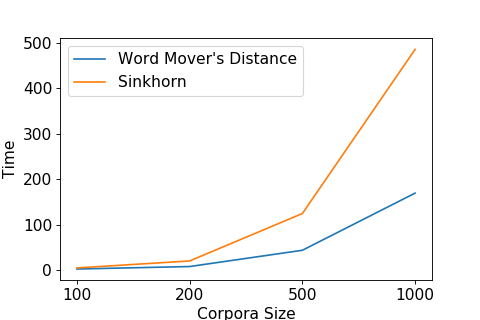
\includegraphics[width=1\linewidth]{perf.png}
    \caption{Timing comparison between word mover's distance and Sinkhorn algorithm}%
    \label{fig:perf}
\end{figure}

\subsection{Supervised Alignment Results}%
\label{sec:supervised_encoding_results}

In order to train our supervised dictionary definition encoder, we used Keras~\cite{chollet_keras_2015}.
All the available definitions were used for this task so refer to Table~\ref{tab:wordnet_stats} for the details on the size of the experiment data.
Romanian wordnet includes the highest number of definitions, followed by Greek and Italian.
Since the task is supervised, we would expect the highest accuracy from those wordnets.

We trained our models over 200 epochs but the accuracy and training loss plateau after 50 epochs so we only report up to \nth{50} epoch on our figures to reflect that.
Due to highest coverage of tokens, we ran the supervised experiments using fastText embeddings, truncated to 1 million tokens.
Learning rate of the model initialized on 1 and adapted dynamically.
The plateau were hit as the learning rate adapted to 0.01.
The input for the network was chosen as 25 words.
Definitions that were longer than 25 words were truncated.
The dimensions of the LSTM layer was selected as 100 which encoded fastText embeddings on 300 dimensions.

We present the training and \emph{validation} accuracy results on Figure~\ref{fig:LSTM_Acc}
The training and validation \emph{loss} are presented in Table~\ref{fig:LSTM_loss}

\begin{figure}[htpb]
    \centering
    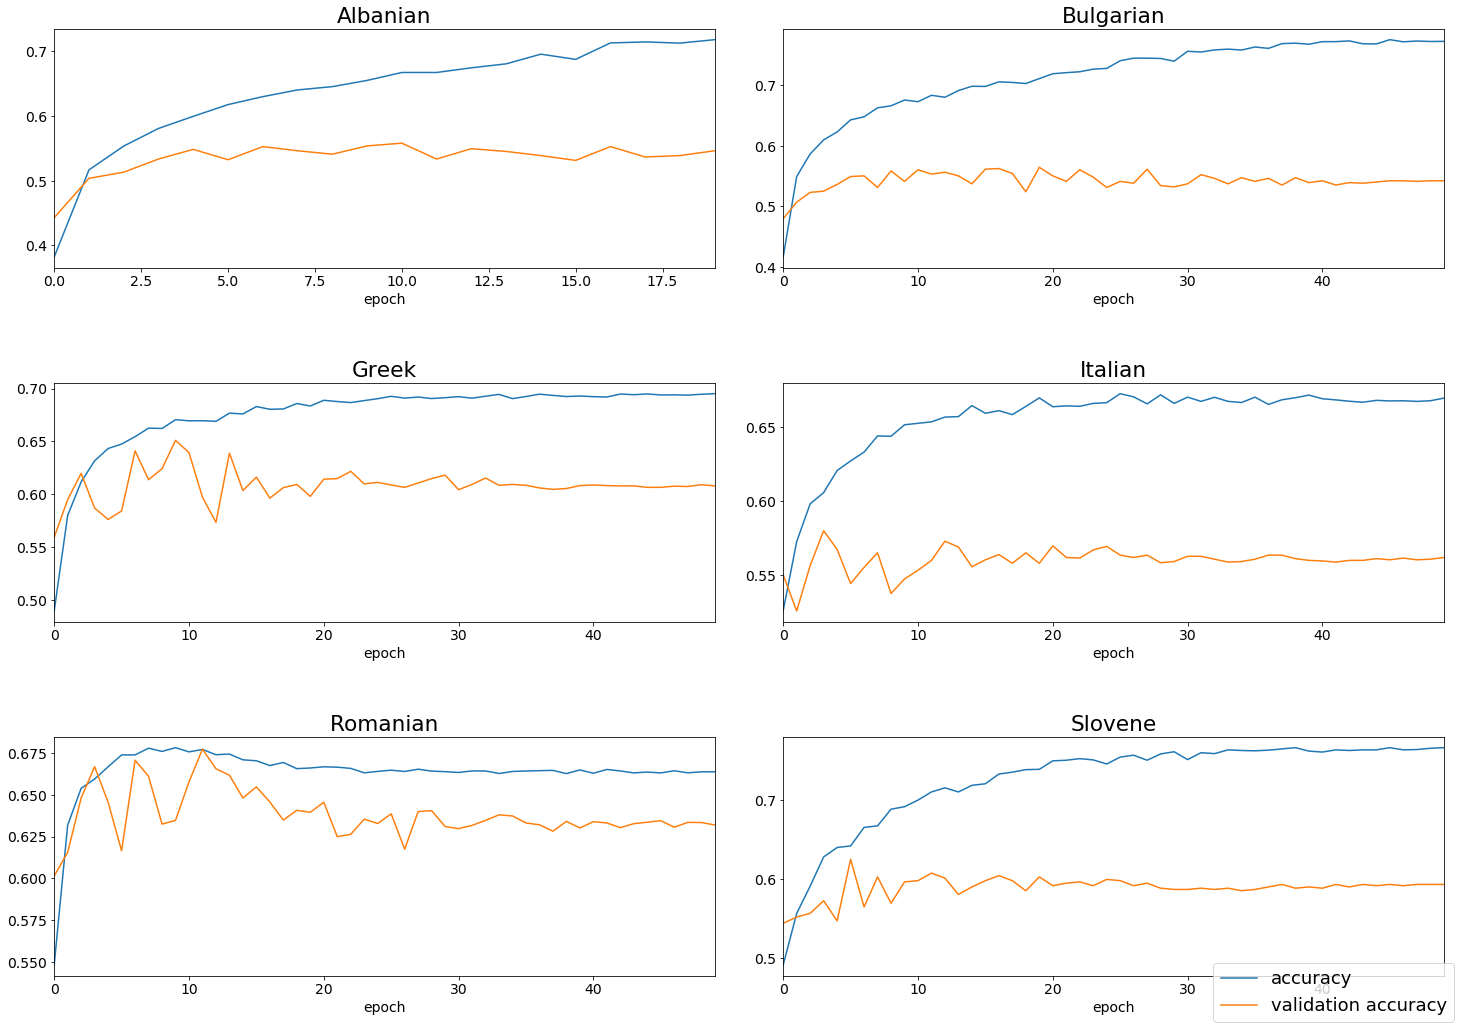
\includegraphics[width=1\linewidth]{LSTM_Acc.png}
    \caption{Accuracy of the supervised encoder on 6 wordnet corpora}%
    \label{fig:LSTM_Acc}
\end{figure}


\begin{figure}[htpb]
    \centering
    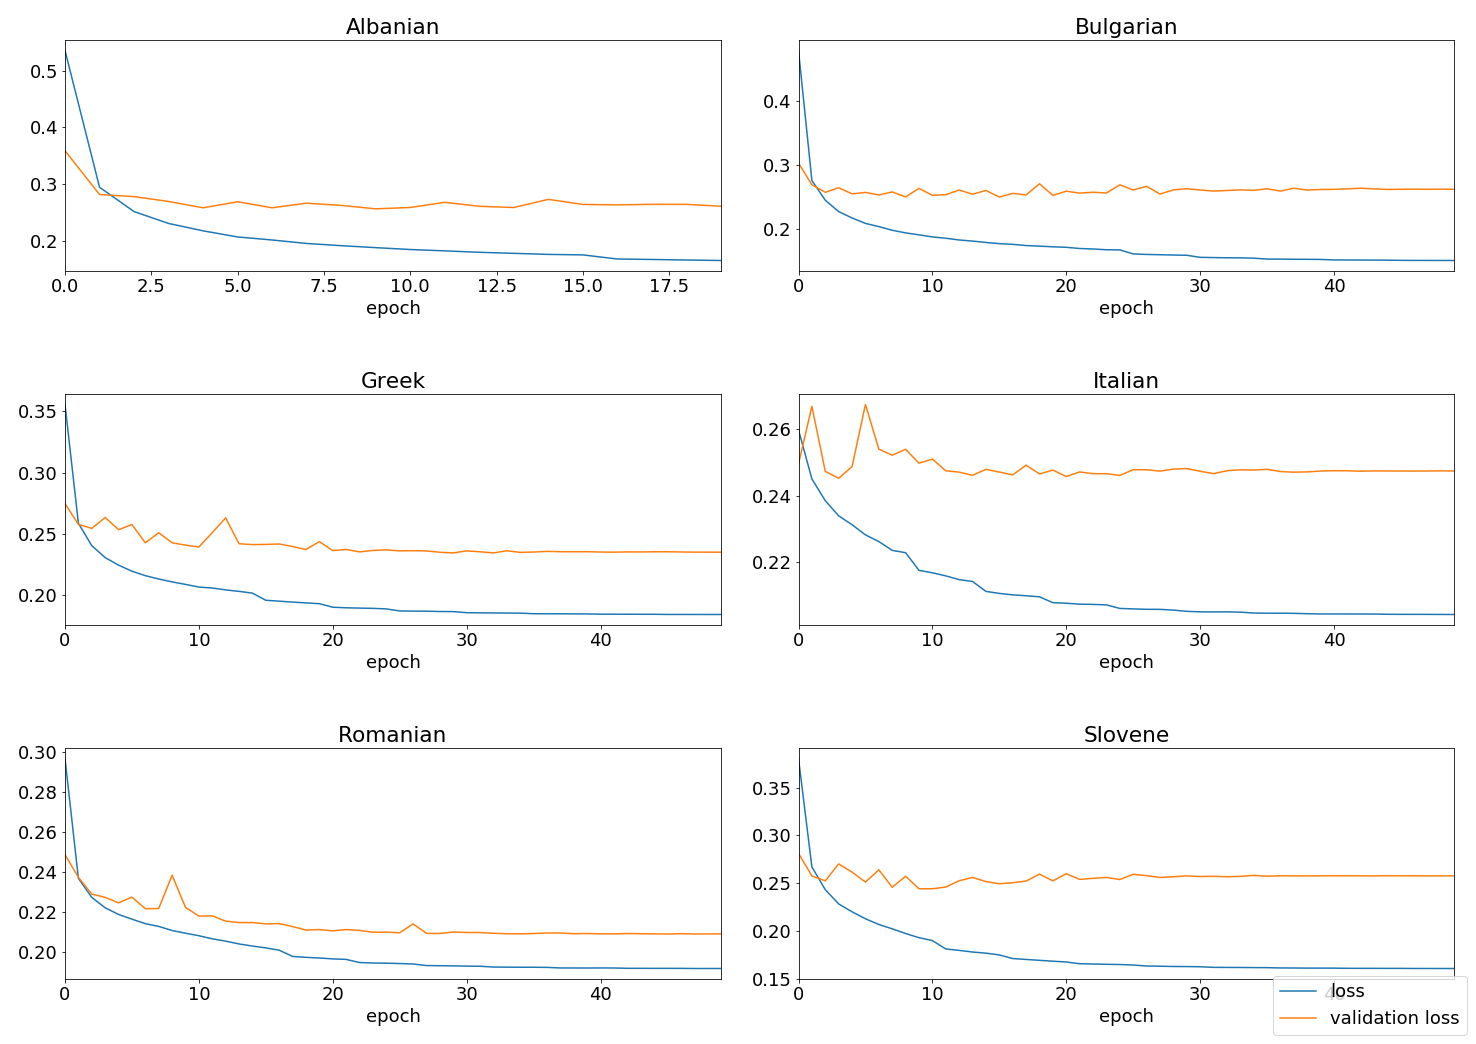
\includegraphics[width=1\linewidth]{LSTM_Loss.png}
    \caption{Loss of the supervised encoder on 6 wordnet corpora}%
    \label{fig:LSTM_loss}
\end{figure}

Overall, we achieved the best validation accuracy, the accuracy on definitions that were never seen in training data with the language that has the highest number of training data avaiable, Romanian.
After 15 epochs of training, accuracy of 65\% is achieved and the accuracy fluctuates around 63\% after \nth{30} epoch.
Surprisingly, the encoder's performance was comparable among Bulgarian and Italian even though the latter has less than half the data available to train than Italian.

\begin{table}[htbp]
    \centering
    \begin{tabulary}{1\linewidth}{L R R}
        \toprule
        Language Code & Dictionary Size & Accuracy After Plateau  \\
        \midrule
        bg & 4959 & 0.56  \\
        el & 18136 & 0.60  \\
        it & 12688 & 0.56  \\
        ro & 58754 & 0.64  \\
        sl & 3144 & 0.59  \\
        sq & 4681 & 0.53 \\
        \bottomrule
    \end{tabulary}
    \caption{The relation between the validation accuracy and the number of data points}%
    \label{tab:lstm_size_acc}
\end{table}


%%%%%%%%%%%%%%%%%%%%%%%%%%
%  IN DOMAIN EMBEDDINGS  %
%%%%%%%%%%%%%%%%%%%%%%%%%%
\section{Investigating Word Embedding Sources}%
\label{sec:investigating_word_embedding_sources}

We also experimented with \emph{fastText} embeddings that were trained using the data available to us.
The research question we are aiming to answer is if pre-trained embeddings are better than embeddings trained on the experiment data.
Since Romanian wordnet has the most data available and word embedding's distributional models perform better as they learn from more distributional information, we have trained Romanian embeddings on the Romanian wordnet definitions.
English fastText embeddings are trained on English Princeton WordNet definitions that were in the experiment set of Romaian wordnet.
Then we mapped the embeddings to the same latent space using supervised VecMap and ran cross lingual document retrieval experiments using word mover's distance and Sinkhorn.
Compared to MRR score of 51.30 for the word mover's distance and 51.95 with the Sinkhorn algorithm, using word embeddings trained using available data resulted in an MRR score of 28.69 for word mover's distance and 28.6 for Sinkhorn.
Considering the drop in performance, we did not repeat the experiments for other language's corpora.

\section{Comparative Analysis}%
\label{sec:comparative_analysis}

In this section, we will compare the matching and the retrieval approaches by exploring the usage of metrics that were discussed on opposite sections.
In other words, we \emph{retrieved} dictionary definitions on the basis of cosine similarity between sentence embeddings of the dictionary definitions and \emph{matched} dictionary definitions using word mover's and Sinkhorn distances as the edge weights of the bipartite graph.

In order to draw accurate conclusions, both matching and retrieval approaches were run on two sets constrained to 2000 dictionary definitions.
Only fastText vectors that were truncated to most frequent 500 thousand (or fastText 500k in the context of this chapter) is used.
Further, we only report \emph{precision at one} or the percentage of correctly matched definitions in order to compare retrieval and matching approaches fairly.
For cross lingual pseudo document retrieval, word mover's distance and Sinkhorn algorithms that use term definition matrices that were weighted using term frequency (Refer to Table~\ref{tab:cldr_pao}) consistently perform worse than \tfidf{} weighted variants so they are not included in the comparisons.

We have split the presentation in two due to size constraints.
Table~\ref{tab:comparison_retrieval} is the overview of the retrieval approaches.
Using a metric to represent dictionary definitions and a similarity measure between them, given a query definition from target language, English Princeton WordNet definitions are ranked according to the similarity metric.
The evaluation is the percentage of queries where English definition with the same index as the query is ranked on top.
\textcite{balikas_cross-lingual_2018} proposed using word mover's and Sinkhorn distances in order to retrieve documents in a different language than the query.
Their state of the art model achieved the highest precision among the retrieval approaches we studied.

Using sentence embeddings in the context of matching is discussed in detail at Section~\ref{sec:linear_assignment_using_sentence_embeddings}.
Extending said approach using word mover's distance or Sinkhorn distance is trivial.
First, both metrics are used to populate a definition to definition distance matrix where $w_{i,j}$ is the distance calculated by either algorithm, between a term $i$ of source language and a term $j$ of the target language.
Jonker-Volgenant algorithm is run in order to find the assignment where the overall sum of the distances is minimized.
This approach is evaluated on the percentage of matched definitions with the same index.
Table~\ref{tab:comparison_matching} presents the evaluation of matching approaches.

Looking a Table~\ref{tab:comparison_matching}, \textbf{Sinkhorn} distance is the best performing metric.
On Table~\ref{tab:showdown}, best precision at one percentage scores for retrieval and matching approaches are presented.
Apart from the retrieval using word mover's distance on English and Albanian dictionary defintions, every score belongs to a metric that used Sinkhorn distance.
Furthermore, matching has a clear advantage over the retrieval approaches.

\begin{table}[p]
    \centering
    \begin{tabulary}{1.0\textwidth}{L R R R R}
        \toprule
        \multicolumn{1}{c}{} & \multicolumn{4}{c}{Precision at one \%} \\ \cmidrule(l){2-5}
        \textbf{Language Code} & \textbf{WMD tfidf} & \textbf{Sinkhorn tfidf} & \textbf{Sentence Embedding} & \textbf{Google Translate Baseline} \\ \midrule
        bg & 41.90 & \textbf{43.00} & 8.60 & 20.15 \\
        el & 38.45 & \textbf{39.95} & 12.40 & 35.45 \\
        it & 31.15 & \textbf{31.30} & 10.45 & 12.50 \\
        ro & 41.65 & \textbf{42.20} & 14.70 & 36.40 \\
        sl & 17.80 & \textbf{17.95} & 6.05 & 15.85 \\
        sq & \textbf{58.70} & 56.85 & 10.65 & 38.35 \\ \bottomrule
    \end{tabulary}
    \caption{Comparison of the \textbf{retrieval} approaches presented in the study}%
    \label{tab:comparison_retrieval}
\end{table}

\begin{table}[p]
    \centering
    \begin{tabulary}{1.0\textwidth}{L R R R}
        \toprule
 & \multicolumn{3}{c}{Precision at one \%} \\ \cmidrule(l){2-4}
        \textbf{Language Code} & \textbf{WMD tfidf} & \textbf{Sinkhorn tfidf} & \textbf{Sentence Embedding} \\ \midrule
        bg & 49.95 & \textbf{51.35} & 40.75 \\
        el & 65.65 & \textbf{66.00} & 37.70 \\
        it & 39.45 & \textbf{39.50} & 28.25 \\
        ro & 67.60 & \textbf{68.20} & 39.45 \\
        sl & 28.16 & \textbf{30.08} & 15.05 \\
        sq & 79.55 & \textbf{79.65} & 54.15 \\ \bottomrule
    \end{tabulary}
    \caption{Comparison of the \textbf{matching} approaches presented in the study}%
    \label{tab:comparison_matching}
\end{table}

\begin{table}[p]
    \centering
    \begin{tabulary}{1.0\textwidth}{L R R}
        \toprule
 & \multicolumn{2}{r}{\textbf{Precision at one \%}} \\ \cmidrule(l){2-3}
        \textbf{Language Code} & \textbf{Retrieval} & \textbf{Matching} \\ \midrule
        bg & 43.00 & 51.35 \\
        el & 39.95 & 66.00 \\
        it & 31.30 & 39.50 \\
        ro & 42.20 & 68.20 \\
        sl & 17.95 & 30.08 \\
        sq & 56.85 & 79.65 \\ \bottomrule
    \end{tabulary}
    \caption{Direct comparison between best performing matching and retrieval approaches}%
    \label{tab:showdown}
\end{table}

%%%%%%%%%%%%%%%%
%  CASE STUDY  %
%%%%%%%%%%%%%%%%
\section{Case Study}%
\label{sec:case_study}

To observe the performance of dictionary alignment on a real life scenario we acquired a proprietary Turkish dictionary granted solely for research purposes.
After parsing, 67351 headwords spanning 93062 definitions are extracted.
Against 117000 synsets (that correspond to unique definitions) of WordNet, the size of the problem is not feasible due to memory restrictions of the pseudo document retrieval approach.
We have tried to overcome it by running the experiment on only nouns but the issue persisted.
As a result, as suggested by \textcite{khodak_automated_2017}, we constrained our scope to a list of core WordNet synsets.
Open Multilingual Wordnet hosts\footnote{\url{http://compling.hss.ntu.edu.sg/omw/wn30-core-synsets.tab}} a list that denotes 4961 WordNet identifiers in the form of offset and part of speech that is compatible with the nltk library, which was used to access to definitions of the identified synsets.\footnote{\url{http://www.nltk.org/}}
The list has been prepared by \textcite{boyd-graber_adding_2006} with the help of human evaluators by selecting salient synsets from a list of frequent words.
Using a set of core WordNet synsets allowed us to pick a problem domain that can be tackled.

As further suggested by \textcite{khodak_automated_2017}, the identifiers for verbs and adjectives are deleted leaving only nouns.
The final experiment set for Turkish dictionary definitions is prepared by translating the lemmas of the core WordNet synsets to Turkish and using the resulting list of lemmas to query the headwords of the Turkish dictionary.
Using this method, we obtained 601 Turkish definitions. After removing the adjectives and verbs, 3280 WordNet definitions formed the definitions to retrieve against.

The approach for the case study is the word mover's distance using \tfidf{} weights, ran on fastText embeddings prepared using supervised VecMap.
The bilingual dictionary provided by OpenSubtitles is used in order to map Turkish and English fastText embeddings.

While preparing the corpora for the pseudo document retrieval, 101 Turkish definitions are dropped due to them having no words to be represented by fastText embeddings while only 3 English definitions had to be omitted.
Then, pseudo document retrieval is run over 501 Turkish definitions and 3277 English definitions.

In order to report on the performance for this task, we asked people to volunteer on scoring the resulting definition pairs.
100 definition pairs are chosen randomly among the 601 Turkish-English pairs and presented online for human annotators to score.
We reached out to undergraduate students of TED University.
The proficiency in English is required for the institution, so the volunteers should have an adequate grasp on the task.

The scale we presented included 3 scores.
A score of \enquote{1} denoted that two definition pairs are completely unrelated, a score of \enquote{2} was asked if the pair of definitions are related and the score of \enquote{3} should be given for pairs that completely entail each other.
The participants did not fill out every pair of definitions and 2 participants had to be omitted since they simply scored 1 or 3 for every definition pair respectively.
At the end, we achieved 10.26 answers for each definition pair.
Fleiss' Kappa measure~\cite{fleiss_measuring_1971} is employed in order to measure the reliability of the given answers. The answer set scored $\kappa = 0.35$.

\begin{table}[htbp]
    \centering
    \begin{tabulary}{1.0\linewidth}{ C C C}
        \toprule
        \multicolumn{3}{c}{Percentage of Definitions} \\ \cmidrule(){1-3}
        \textbf{Unrelated} & \textbf{Related} & \textbf{Entails} \\
        \cmidrule(rl){1-3}
        49.61 & 25.93 & 24.46 \\ \bottomrule
    \end{tabulary}
    \caption{Results of the case study; percentage of definitions that were agreed on by human annotators}
    \label{tab:case_study_resutlts}
\end{table}

According to the human referees, 24.46\% of definitions completely entails each other while another 25.94\% are related.
However, volunteers marked another 49.61\% of the definitions as unrelated.
In Appendix~\ref{app:case_study}, we present the 100 randomly selected pairs of English definitions that were retrieved as the top result against the respective Turkish query.
